% test.tex
\title{An Analysis Of The Women's Super League}

\author{Ellen M. Leahy}

\newcommand{\abstractText}{\noindent
In this report, I investigate Women's Super League (WSL) data from 2017 to 2022. I will focus on the change of attendance over time, goals and xG per season and per game, and the number of different nationalities represented and how this correlates to team performance. As women's football has grown in popularity over the past number of years, we do see some increase in attendance/ However, this is not widespread across all teams and matches, likely due to teams still playing in small stadia. We also find that the highest performing teams tend to have more international players, suggesting the importance of scouting further afield.
}

%%%%%%%%%%%%%%%%%
% Configuration %
%%%%%%%%%%%%%%%%%

\documentclass[12pt, a4paper, twocolumn]{article}
\usepackage{xurl}
\usepackage[super,comma,sort&compress]{natbib}
\usepackage{abstract}
\usepackage{graphicx}
\renewcommand{\abstractnamefont}{\normalfont\bfseries}
\renewcommand{\abstracttextfont}{\normalfont\small\itshape}

\usepackage[font=small,labelfont=bf]{caption}

\usepackage{pagecolor}% http://ctan.org/pkg/{pagecolor,lipsum}
\usepackage[a4paper, total={6.5in, 8.8in}]{geometry}
\pagecolor{white}

%%%%%%%%%%%%%%
% References %
%%%%%%%%%%%%%%

% Any configuration that should be done before the end of the preamble:
\usepackage{hyperref}
%\hypersetup{colorlinks=true, urlcolor=blue, linkcolor=blue, citecolor=blue}

\begin{document}

%%%%%%%%%%%%
% Abstract %
%%%%%%%%%%%%

\twocolumn[
  \begin{@twocolumnfalse}
    \maketitle
    \begin{abstract}
      \abstractText
      \newline
      \newline
    \end{abstract}
  \end{@twocolumnfalse}
]

%%%%%%%%%%%
% Article %
%%%%%%%%%%%

\section{Data Collection}

The data for this report was taken from the website \verb|www.fbref.com|. FBref is a hub of information for sports data, covering 140 competitions across 45 countries \cite{fbref}. I focused on the Women's Super League (WSL) for this report, which first began in 2017, and I used data until the end of the most recent complete season, 2021-22. 

While there are many datasets available for the Super League, for the purpose of this report I focus on  three: the league overview, scores and fixture data, and player standard stats. Each dataset is discussed in more detail below. The data was obtained by exporting each table for each season as a CSV and copying to my local machine. The data, code and visualisations, along with a copy of these report, can be found on my GitHub page\cite{git}.

\subsection{League Overview}

At a high level, the squad standard data\cite{overview} is simply a league table with one row per team. Included is information about the squad, such as average age and number of players, the number of games played and the performance in those games, including goals and expected goals (xG) per season and per match. xG is a statistical tool to measure the likelihood of a player scoring a particular shot, taking into account the players position on the pitch, what part of their body their shooting with and the type of assist, such as a cross or through ball, amongst other variables\cite{xg}.

There are a few areas where data is missing and some seasons have fewer fixtures than others. Firstly, the 2016-17 season only ran for 3 months, as prior to this the WSL ran throughout the summer, but was changed to follow the same calendar as the men's game. While it occurred between April and June 2017, I have labelled this season 2016-17 for consistency. Prior to the 2018-19 season there was no xG data, so these rows will contain nulls. As the team in last place is relegated at the end of the season, and the winner of the championship takes their place, not every team has played the same number of games overall. Finally, due to the pandemic, the 2019-20 season was ended early and the winner decided on a point per game bases, therefore fewer games were played.

\subsection{Scores and Fixtures}

The second dataset I explored was fixtures data\cite{fixtures}, containing one row per match. This includes data for when the match was held, such as date and time, the home and away teams, the attendance, venue and referee, as well as the score.

Due to the cancelled matches during the pandemic, some games were not played, these rows still exist in the data, however the score column is not populated. See section 2.2 for more information on how this was dealt with. As per the league overview data, xG information was only added from the 2018-2019 season.

\subsection{Player Standard Stats}

Finally, we have data on each player in the Player Standard Stats table\cite{players}. This table contains one row per player who appeared in the WSL that season, this does not include any squad player who did not get any minutes on the pitch. Columns in this dataset include information on the nationality, position and age of the player, the number of matches played and their overall statistics for the season and at match level, including goals and assists. This dataset also only includes xG data from the 2018-2019 season onwards.

\section{Data Cleaning}

For each dataset, the data had to be downloaded individually for each season. In order to make visualisation easier, I combined each season into one larger file, giving one file per table. This is done in the $`combine\_data.py$' script, using the concat function. As the tables are all in CSV format, we are able to read through each folder and automatically concatenate each file into a new dataframe, therefore if a new dataset is added, the script does not need to be changed. I have chosen to save the data in CSV files as this allows for quick reading and writing of data, and is easy to manually inspect.

\subsection{League Overview}

Minimum cleaning was required for this dataset. For easy visualisation, I split the \verb|Top Team Scorer| into two columns: \verb|Top Scorer| and \verb|Top Scorer Num Goals|, and dropped the original column.

\subsection{Scores and Fixtures}

The original format of this table included a header and sub-headers, in the concatenation of these tables, the sub-headers were included as rows. To remove these, we filter out any row where \verb|Score==NaN|. This has the benefit of also removing any matches which were cancelled, which are not interesting and do not add anything to our analysis. Finally, we split the score into two columns, \verb|Home Goals| and \verb|Away Goals| which will make visualisation easier later.

\subsection{Player Standard Stats}

The player standard stats dataset has some non-sense columns, such as \verb|-additional| and \verb|unnamed: 32|, the first step of cleaning is simply removing these. Similarly to the fixture data, the original table had a header and sub-header. The sub-headers contain the name of the variable measured and the header states whether this column measures the value across the season or per 90 minutes, therefore, we need to use a combination of these two values to correctly label each column. By visual inspection, I wrote the following regex statements to deduce whether the column represents the full season or a match respectively: \verb=(^Performance|^Expected)= and \verb=^Per 90.= . Once the columns are named correctly, we can drop the rows which were intended to be sub-headers and output to a new CSV file.

\section{Analysis}

In analysing the data, I focus on four measures: attendance, goals, xG and number of distinct nationalities. In each, I will use a combination of the datasets to explore the data, primarily through visualisations. The tools used were Matplotlib, Pandas, Numpy, Colorsys and SciPy.

\subsection{Attendance}

In recent years, particularly since the world cup in 2019, women's football has seen a surge in popularity. I hypothesise that this would lead to an increase in attendance in the WSL. Firstly, we will use the League Overview data to look at the average attendance per season, see Figure \ref{avg_att}. As expected, we see a sharp increase in attendance following the 2019 world cup, we also see a sharp drop off in the 2020-21 season where fans were not permitted to attend due to the Coronavirus pandemic. 

\begin{figure}
  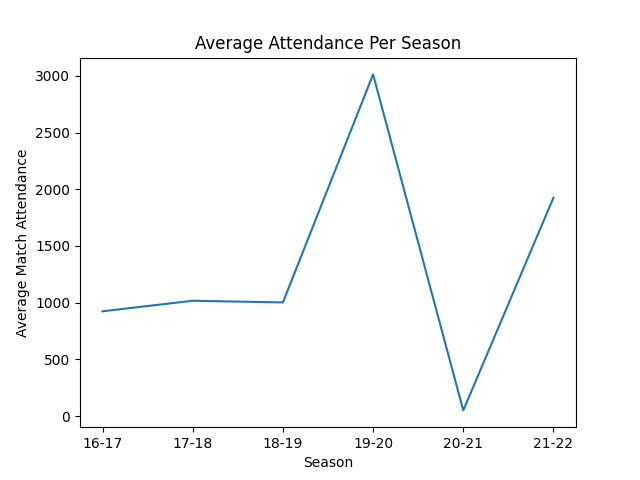
\includegraphics[width=\linewidth]{../vis/tables/average_attendance.png}
  \caption{Average Attendance Per Season.}
  \label{avg_att}
 \end{figure}

However, this graph does not tell us whether there was an overall increase in attendance or if there were outliers increasing the average. To answer this question, I plot a box and whisker chart showing the variation of average attendance for each team per season, see Figure \ref{att_box}. This shows us that while the median and upper whisker has increased significantly, the lowest attended games have only increased slightly. Furthermore, the attendance did not jump back up to pre-pandemic figures as one might have hoped in the 2021-22 season.

\begin{figure}
  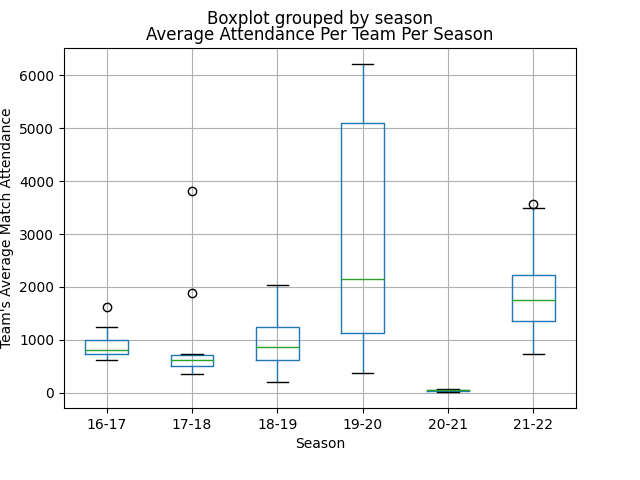
\includegraphics[width=\linewidth]{../vis/tables/attendance_boxwhisker.png}
  \caption{Box and whisker chart showing attendance per season.}
  \label{att_box}
\end{figure}

Using the fixtures data, we can get a more granular view of how attendance has changed over time. Figure \ref{att_ot} shows the highest attended match per day in the WSL. I chose the maximum rather than the sum as this will remove any bias from days where multiple games were played. From Figure \ref{att_ot}, we can see that there have been a handful of games which have had a very high attendance, but at first glance it appears that the overall attendance hasn't shown a significant increase.

\begin{figure}
  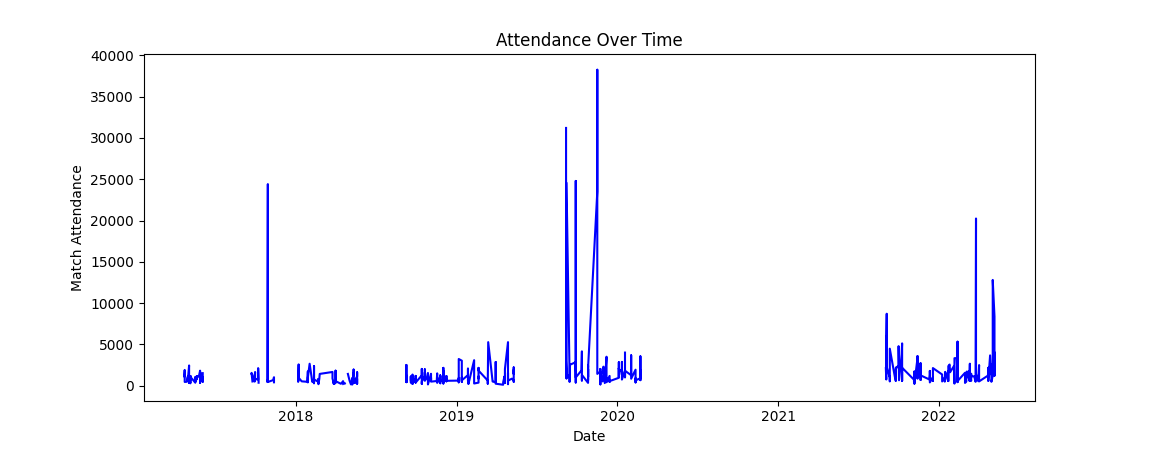
\includegraphics[width=\linewidth]{../vis/fixtures/attendance_overtime.png}
  \caption{Line chart showing attendance over time.}
  \label{att_ot}
\end{figure}

In order to test this theory, I removed the outliers from the data and re-plot the graph. For the purposes of this analysis, I have defined the outliers as any point above the upper outer fence, given by
\begin{equation}
 Q_3 + 3 \times h\_spread
\end{equation}
where the \textit{h-spread} is defined by the difference between the first and third quartile and $Q_3$ is the third quartile. We will not consider the outliers on the lower limit as these are not relevant for our analysis. I replaced each outlier with \verb|NaN| and the new plot is shown in Figure \ref{att_ot_noout}. From this, we can see that there has been a general increase in attendance in the WSL, however there are still many games with a very low attendance, I suspect this is caused by some clubs pushing for a higher attendance more than others.

\begin{figure*}
  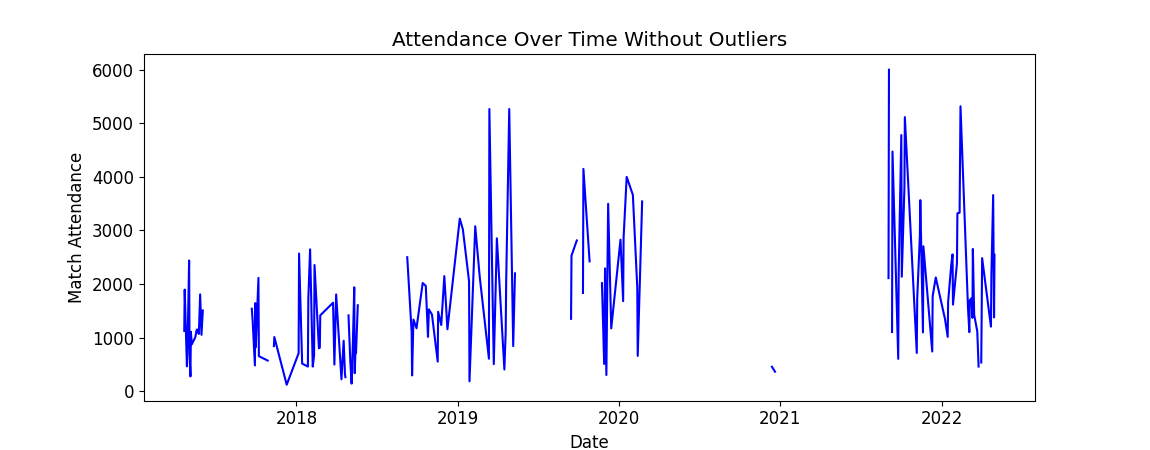
\includegraphics[width=\linewidth]{../vis/fixtures/attendance_overtime_no_outliers.png}
  \caption{Line chart showing attendance over time, with outliers removed.}
  \label{att_ot_noout}
\end{figure*}

Finally, we ask the question `does attendance even matter'? As fans, we often believe that our presence can help our team perform better, so lets investigate this hypothesis. For these purposes, I will use goals as a proxy for performance. Using the fixtures data, I plot goals scored by the home and away teams against attendance, as we would assume that the majority of the crowd are supporting the home team. Figure \ref{att_v_goals} shows that a higher attendance does not correlate to more goals scored by either the home or the away team, in fact the highest scoring games are the lowest attended. This is likely because the top teams will only host their `big' games in larger stadia, as they believe these will attract more fans. This will lead to fewer goals being scored as both teams have a strong defence when compared to the weaker teams at the bottom end of the table. To truly understand the effect of the crowd, we would need each team to play all of their games in a single ground across the season.

\begin{figure*}
  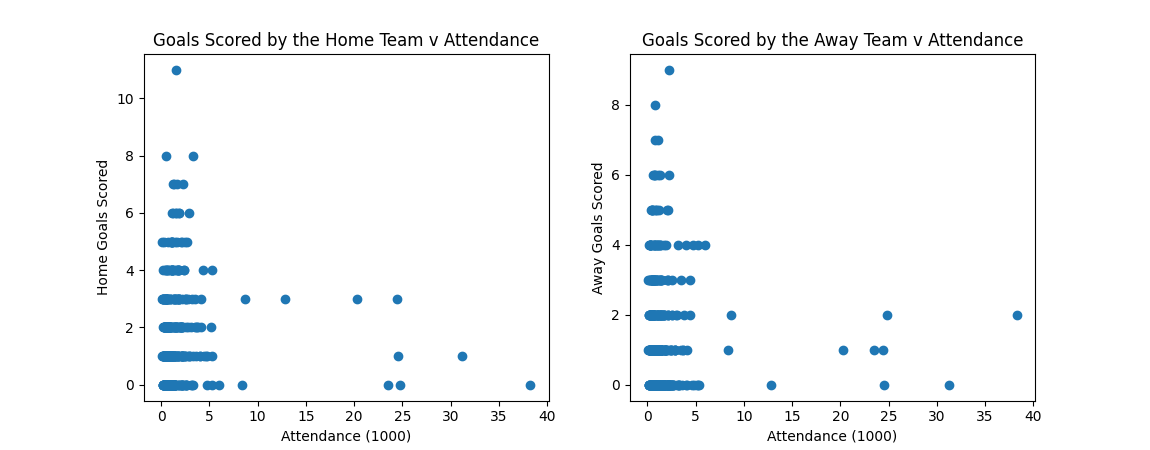
\includegraphics[width=\linewidth]{../vis/fixtures/attendance_v_goals.png}
  \caption{Home (left) and away (right) goals scored v attendance}
  \label{att_v_goals}
\end{figure*}

\subsection{Goals}

In this section, we will investigate the correlation between minutes played and goals scored, we will also dig into who the league's top scorers are. Firstly, Figure \ref{goal_min} shows the number of goals scored against the minutes played, coloured by position, created using the players data so the results is at season level. Overall, there is not a significant trend between the two, however when we look at only forwards, red, there does seem to be a correlation.

\begin{figure}
  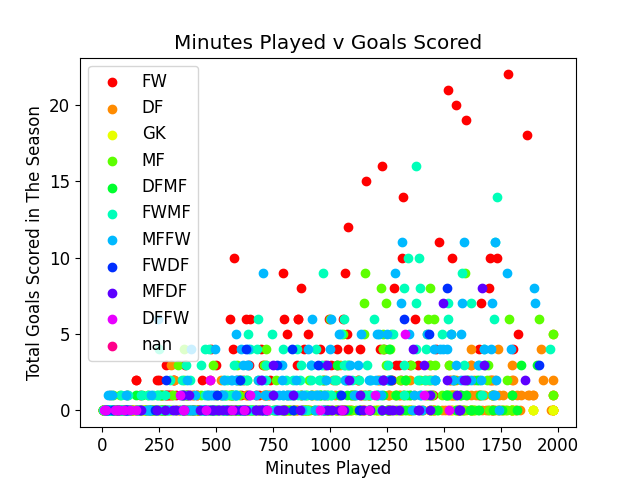
\includegraphics[width=\linewidth]{../vis/playerStats/goal_minutes}
  \caption{The number of goals scored by a player v minutes played per season, coloured by position.}
  \label{goal_min}
\end{figure}

To confirm this, we can plot only the forwards, see Figure \ref{goal_min_fw}. We can see that, even for forwards, there are many players who play a significant number of minutes in the season and score very few goals. In fact, for the majority of players, the number of goals appears uncorrelated to the number of minutes. I have added labels to the players who have scored the top 5\% of goals in a season, interestingly we see Vivianne Miedema (Arsenal) and Sam Kerr (Chelsea) appear three times and twice respectively, with one appearance from Nikita Parris (Manchester City). As these players have scored the most in a single season, we would expect them to be some of the highest scoring players in the history of the WSL.

\begin{figure}
  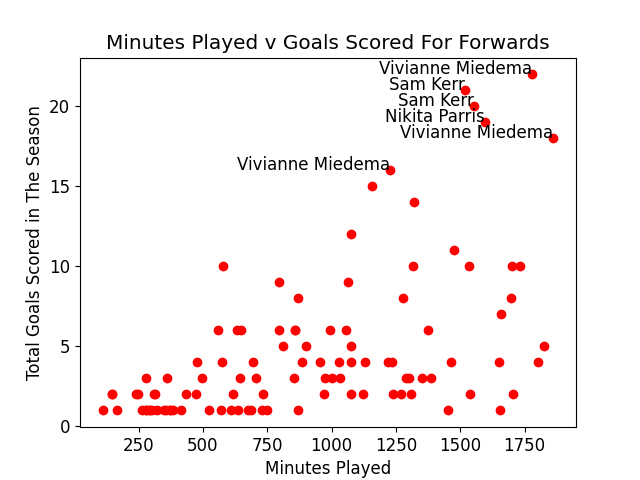
\includegraphics[width=\linewidth]{../vis/playerStats/goal_minutes_forwards.png}
  \caption{The number of goals scored by a forwards v minutes played per season.}
  \label{goal_min_fw}
\end{figure}

Figure \ref{top_scorers} shows the top ten players ranked on the total number of goals and assists provided in the WSL since its creation. Unsurprisingly from the previous chart, Miedema is ranked number one, however Kerr is only sixth. This is likely because Kerr only joined the WSL in January 2020, whereas Miedema has been in the league since its conception. 

\begin{figure}
  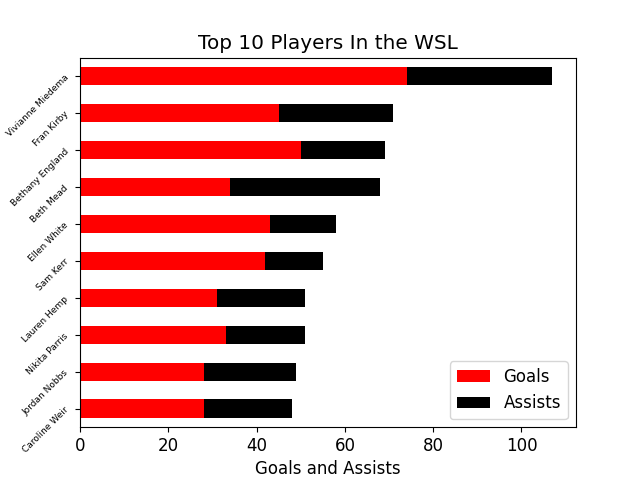
\includegraphics[width=\linewidth]{../vis/playerStats/top_scorers.png}
  \caption{The top ten players by goals and assists in the WSL.}
  \label{top_scorers}
\end{figure}

When we look at goals and assists per season played, Miedema is still top, however Kerr is now up to second, behind her by only a handful of goals. Kerr and Miedema are clearly a step above the rest of the players, with both players scoring more goals than any other player has goals and assists combined.

\begin{figure}
  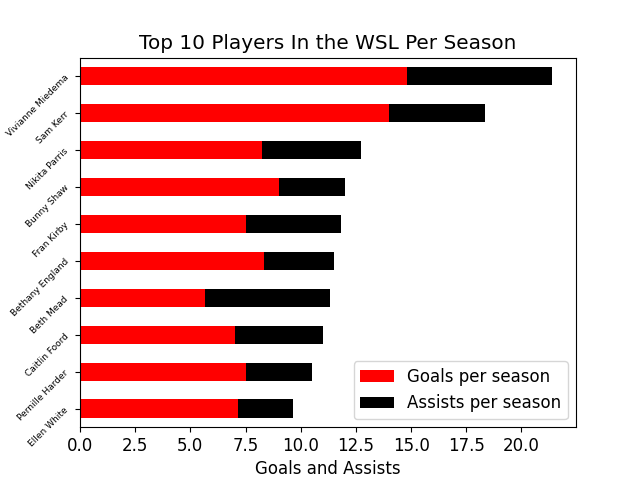
\includegraphics[width=\linewidth]{../vis/playerStats/top_scorers_perseason.png}
  \caption{The top ten players by goals and assists in the WSL per season played.}
  \label{top_scorers_persseason}
\end{figure}

\subsection{Expected Goals (xG)}

Figure \ref{xg} shows the average xG per season. As previously stated we only have xG data from 2018-19 onwards so previous seasons have been filtered out from this section. To calculate average xG, I simply took the final xG value for each team from the \verb|League Overview| dataset, and took its average when aggregated at season level. It appears that the 2019-2020 season had significantly lower xG than other seasons, however, this is likely due to the pandemic causing cancellations.

\begin{figure}
  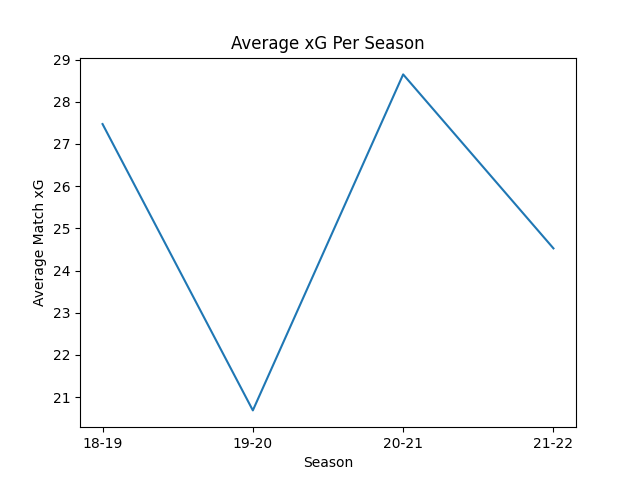
\includegraphics[width=\linewidth]{../vis/tables/average_xg.png}
  \caption{The average xG per season.}
  \label{xg}
\end{figure}

In order to verify this, we can calculate the average xG per game using the \verb|Matches Played| (MP) column, see Figure \ref{xg_pergame} for the resulting graph. We can now see that in fact the 2019-20 season has the highest xG per game. However, this chart is still misleading as there appears to be a significant difference between the xG in 2019-20 and 2021-22. This is caused by the axis ticks starting at 1.10 rather than 0, which we would assume when glancing at the chart. Figure \ref{xg_axis} shows the same chart but with the y-axis now starting at 0, and we can now clearly see that while there was a drop off in xG after the 2019-20 season, it is not as significant as it first appeared.

\begin{figure}
  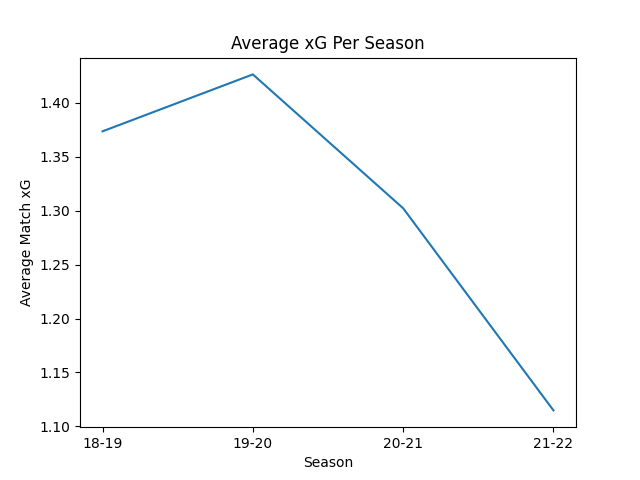
\includegraphics[width=\linewidth]{../vis/tables/average_xg_pergame.png}
  \caption{The average xG per game per season.}
  \label{xg_pergame}
\end{figure}

\begin{figure}
  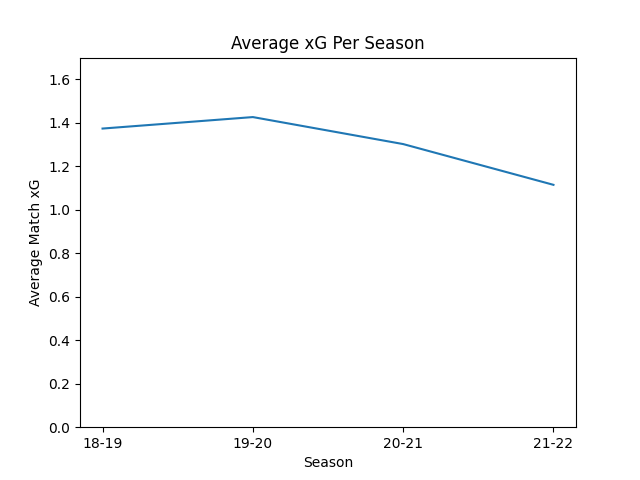
\includegraphics[width=\linewidth]{../vis/tables/average_xg_pergame_newaxis.png}
  \caption{The average xG per game per season with corrected y-axis.}
  \label{xg_axis}
\end{figure}

From Figure \ref{xg_axis}, it is unclear whether the 2019-20 season has a higher xG because there were fewer games and the xG drops naturally over the season or if the xG was just higher compared to other seasons for another reason. To answer this, we can compare the average xG for each match day per season, see Figure \ref{xg_match}. As this chart was very noisy, I used the scipy library to interpolate between points to make a more readable chart. I chose to interpolate with 20 equally spaced values along the x-axis, as this gave the clearest lines which still followed the shape of the raw data (see GitHub\cite{git} for charts at other levels of interpolation). From Figure \ref{xg_match}, we can see that the xG for the 2019-20 season was higher for the same portion of the season compared to other seasons. In general, the xG tends to remain broadly flat across the season, however it is quite variable. Note that the 2018-19 season appears shorter as there were fewer teams, and the 2019-20 season finished early due to the pandemic.

\begin{figure}
  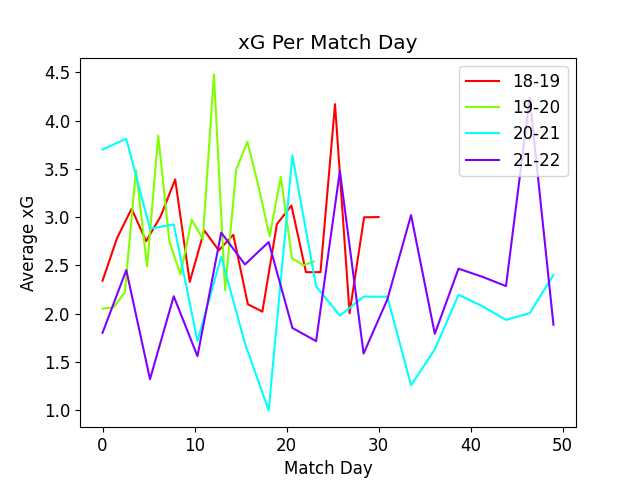
\includegraphics[width=\linewidth]{../vis/fixtures/xg_matchday20.png}
  \caption{Interpolated average xG per match day for each season.}
  \label{xg_match}
\end{figure}

As xG is so closely related to goals, we would expect to see a strong correlation between the two values. To test this, I have used the polyfit function in Numpy to fit a line to the graph of goals scored against xG created per player per season, using the players dataset, see Figure \ref{xg_line}. This looks like a relatively good fit, however, we can verify this by plotting the residuals on a histogram, see Figure \ref{res}. The majority of the residuals are close to zero, showing a reasonable fit, although it is not symmetrical.

Another method of validation is using the reduced chi-square value. The chi-square is given by the equation
\begin{equation}
\sum_{i=1}^n \frac{(E_i - O_i)^2}{E_i} 
\end{equation}
where $E_i$ and $O_i$ are the expected and observed values of goals scored respectively, and the sum is across the number of values in the array. We then divide this result by the number of degrees of freedom, giving us a reduced chi-square value of 0.185, suggesting that these values are strongly correlated.

\begin{figure}
  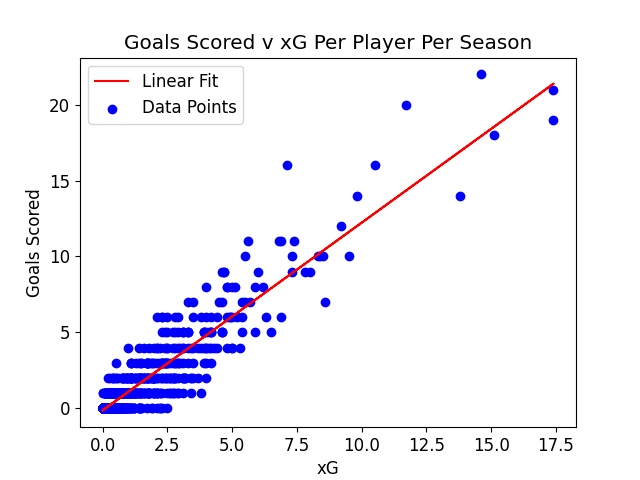
\includegraphics[width=\linewidth]{../vis/playerStats/goals_v_xg_linear_fit.png}
  \caption{A first order fit to the number of goals scored by a player versus the total xG accumulated in a season.}
  \label{xg_line}
\end{figure}

\begin{figure}
  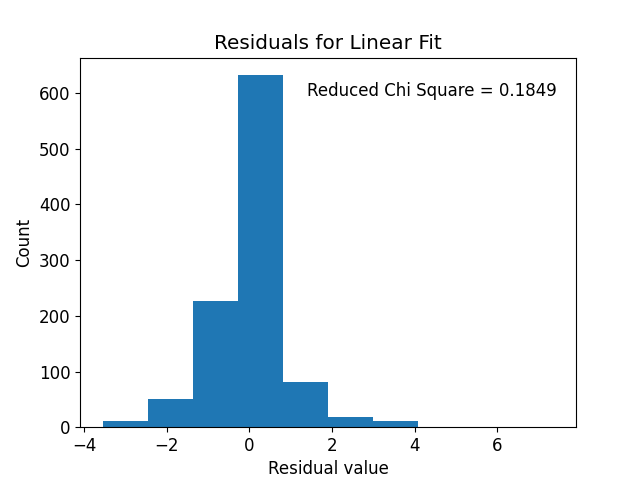
\includegraphics[width=\linewidth]{../vis/playerStats/goals_v_xg_residuals.png}
  \caption{Residual values for the linear fit of xG versus Goals.}
  \label{res}
\end{figure}

\subsection{Nationalities}

We have grown accustomed to seeing so many nationalities represented in the premier league, we might ask if we see the same in the WSL. Figure \ref{nation_bar} shows the number of players representing each nation. Immediately, we can see that there are far more players from England than any other nation. In fact, it looks like there could be more players from England than all other nations combined.

\begin{figure}
  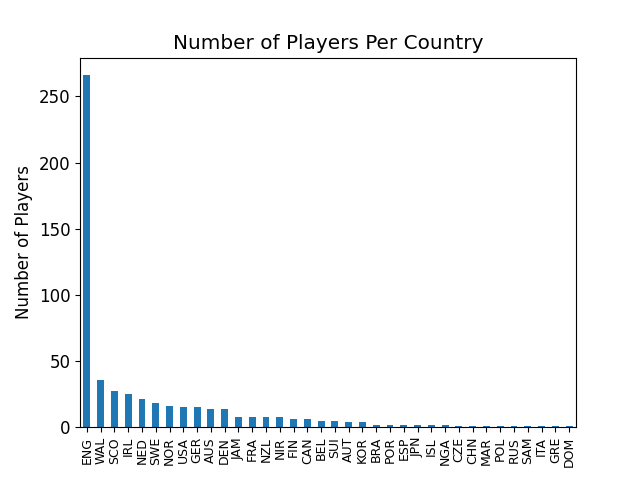
\includegraphics[width=\linewidth]{../vis/playerStats/nation_bar.png}
  \caption{The number of players who have played in the WSL for each nation.}
  \label{nation_bar}
\end{figure}

Figure \ref{nation_pie} helps us to test this hypothesis. This shows that 51.6\% of players in the WSL are not English, a small proportion when compared with the premier league, where 64\% of players who played in the 2021-22 season represented other nations\cite{foreign}. 

\begin{figure}
  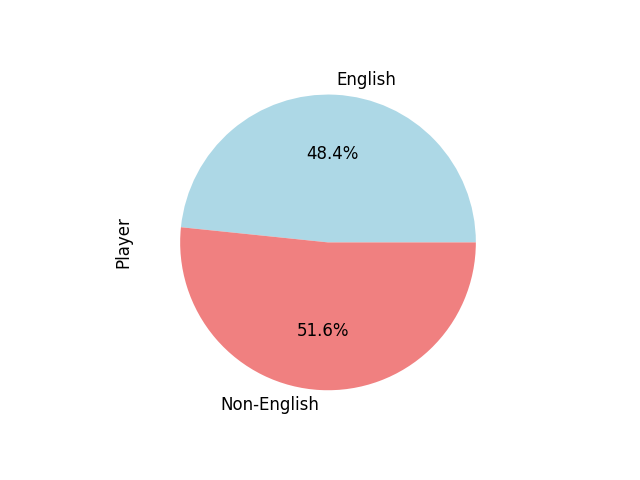
\includegraphics[width=\linewidth]{../vis/playerStats/nation_pie.png}
  \caption{Pie chart showing the number of English versus Non-English players in the WSL.}
  \label{nation_pie}
\end{figure}

One hypothesis for this is that it is more costly and challenging to recruite players from overseas, and as the WSL was created more recently and has significantly less funding than the men's equivalent, clubs can not afford this extra cost. To test this hypothesis, Figure \ref{nation_rank} shows the average squad rank at the end of the season against the number of non-English players the team has. This was calculated by joining the player data to the league overview data. While the relationship is weak, we can clearly see that the teams finishing near the top of the table have more non-English players than the lower ranked teams, which supports my hypothesis.

\begin{figure}
  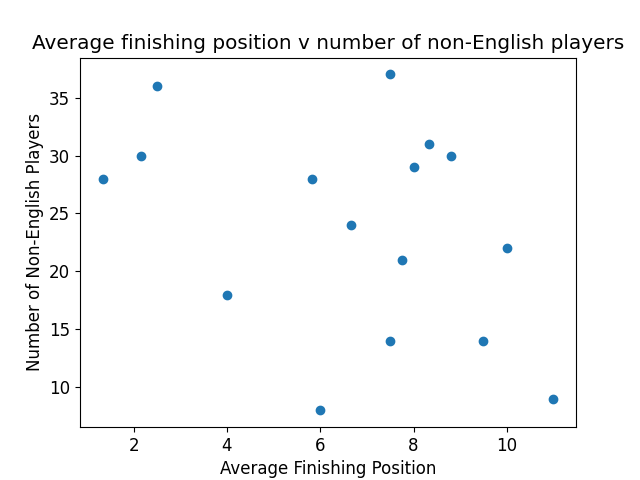
\includegraphics[width=\linewidth]{../vis/playerStats/nation_rank.png}
  \caption{The number of non-English players v the average final league position per team.}
  \label{nation_rank}
\end{figure}

\section{Conclusion}

Overall, I believe my analysis resulted in a number of interesting insights. While women's football has increased in popularity in recent years, this has not been particularly reflected in the attendance, however there are some matches which are attended very highly. If given more data, I would like to calculate the number of sold out games, when played in smaller stadia. Unfortunately, these women are still playing matches in stadia with capacities of only a couple of thousand, we need the clubs to support a move to larger stadia so we can get more fans in.

I found that increased attendance in matches does not lead to more goals being scored, and in fact at matches with greater than 10000 attendees, no team has scored more than three goals. There are many other factors which could lead to this however, including better teams playing in larger stadia, thus having better defences. Furthermore, for the majority of players, playing more minutes does not correlate with scoring more goals, although the top goal scorer have played more minutes in a season. However, a team's top striker is likely to play as many games as possible, regardless of how many goals they are scoring. I also found that the xG has remained broadly flat across the seasons, and within each season, thus, if the attack has been improving, the defence is improving to match it.

Finally, the relationship between a team's final league position and the number of non-English players who played for them shows the benefits of teams being able to look further afield for new players. England, for many years, have lagged behind other nations in the development of women's footballers; USA, the Netherlands and Spain, to name a few, have produced many top talents who have won competitions for their country and club alike. In fact, an English team hasn't won the Champions League since 2006-07, when Arsenal won the quadruple, and England only won their first major honour last summer at the Euros. While there is a long term benefit to improving local academies and facilities, in the short-term, teams need the funding to scout and buy players from overseas.

%%%%%%%%%%%%%%
% References %
%%%%%%%%%%%%%%

\begin{thebibliography}{10}
\bibitem{fbref} FBref, 2023, \textit{FBref}, \date{January 7, 2023}, \textlangle https://fbref.com/en/about \textrangle
\bibitem{git} GitHub, 2023, \textit{GitHub}, \date{January 16 2023}, \textlangle https://github.com/ellenleahy95/
MTH765P\_project \textrangle
\bibitem{xg} Tippet, J 2019, \textit{The xG Philosophy}, self-published
\bibitem{overview} FBref, 2023, \textit{Squad Standard Stats}, \date{December 11, 2022}, \textlangle  https://fbref.com/en/comps/189/2021-2022/stats/2021-2022-Womens-Super-League-Stats\#stats\_squads\_standard\_for \textrangle
\bibitem{fixtures} FBref, 2023, \textit{Squad Standard Stats}, \date{December 11, 2022}, \textlangle  https://fbref.com/en/comps/189/2021-2022/schedule/2021-2022-Womens-Super-League-Scores-and-Fixtures\#sched\_2021-2022\_189\_1 \textrangle
\bibitem{players} FBref, 2023, \textit{Squad Standard Stats}, \date{December 11, 2022}, \textlangle  https://fbref.com/en/comps/189/2021-2022/stats/2021-2022-Womens-Super-League-Stats\#stats\_standard \textrangle
\bibitem{foreign} Transfrmarkt, 2023, \textit{Used Foreign Players}, \date{January 11, 2023}, \textlangle   \verb|https://www.transfermarkt.com/| \verb|premier-league/legionaereeinsaetze/| \verb|wettbewerb/GB1/plus/1?option=|spiele \verb|&saison\_id=2021\=&altersklasse=alle| \textrangle
\end{thebibliography}

\end{document}

% Create PDF on Linux:
% FILE=test; pkill -9 -f ${FILE} &>/dev/null; rm -f ${FILE}*aux ${FILE}*bbl ${FILE}*bib ${FILE}*blg ${FILE}*log ${FILE}*out ${FILE}*pdf &>/dev/null; pdflatex -halt-on-error ${FILE}; bibtex ${FILE} && pdflatex ${FILE} && pdflatex ${FILE} && (xdg-open ${FILE}.pdf &)